\documentclass{article}
\usepackage{graphicx} % Required for inserting images
\usepackage{svg}
\usepackage{booktabs}

\title{Arabic\_data\_description\_0707version}
\author{Linhai Ma}
\date{July 2026}

\begin{document}

\maketitle


\section{Summary of Text File--Metadata Matching}

  We matched the deidentified text files to the metadata using the numeric ID stored as the final underscore-delimited block in each text filename. This ID was matched
  against the \texttt{matched\_ids} column in the metadata. The target labels are columns AO--AS.

  \begin{table}[htbp]
  \centering
  \begin{tabular}{lr}
  \toprule
  \textbf{Item} & \textbf{Count} \\
  \midrule
  Total deidentified text files & 987 \\
  \midrule
  Text files matched to metadata via \texttt{matched\_ids} & 545 \\
  Text files not found in metadata \texttt{matched\_ids} & 442 \\
  \midrule
  Matched IDs with exactly one metadata row & 374 \\
  Matched IDs with multiple metadata rows & 171 \\
  \midrule
  Duplicate IDs with identical labels & 154 \\
  Duplicate IDs with at least one conflicting labels & 17 \\
  \midrule
  Usable text-file IDs with unambiguous labels & 528 \\
  \bottomrule
  \end{tabular}
  \caption{Summary of matching results between deidentified text files and metadata.}
  \label{tab:matching-summary}
  \end{table}

  The 545 matched text-file IDs should not be interpreted as 545 clean usable samples. Among them, 171 IDs matched more than one metadata row. After checking AO--AS
  consistency, 154 duplicated IDs had identical labels and 17 had conflicting labels. Under the strict rule of keeping only unambiguous labels, the usable dataset
  contains:
  \[
  374 + 154 = 528
  \]
  text files.

  \section{Distribution of Target Labels in the Usable Dataset}

  The label distributions for the 528 usable text files are shown in Figures~\ref{fig:wish-to-be-dead}--\ref{fig:specific-plan-intent}. The corresponding count summary
  is shown in Table~\ref{tab:label-distribution-summary}.

  \begin{figure}[htbp]
  \centering
  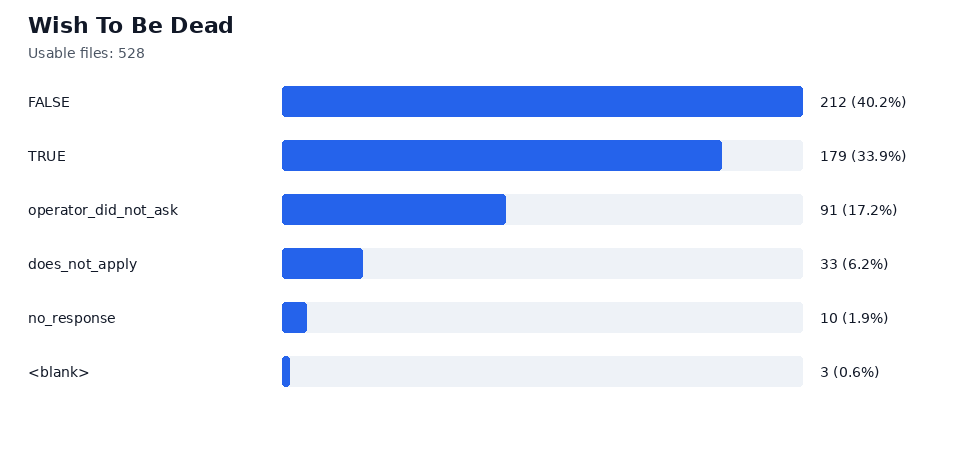
\includegraphics[width=0.95\linewidth]{usable_matches_distribution_plots/wish_to_be_dead.png}
  \caption{Distribution of labels for \textit{Wish To Be Dead}.}
  \label{fig:wish-to-be-dead}
  \end{figure}

  \begin{figure}[htbp]
  \centering
  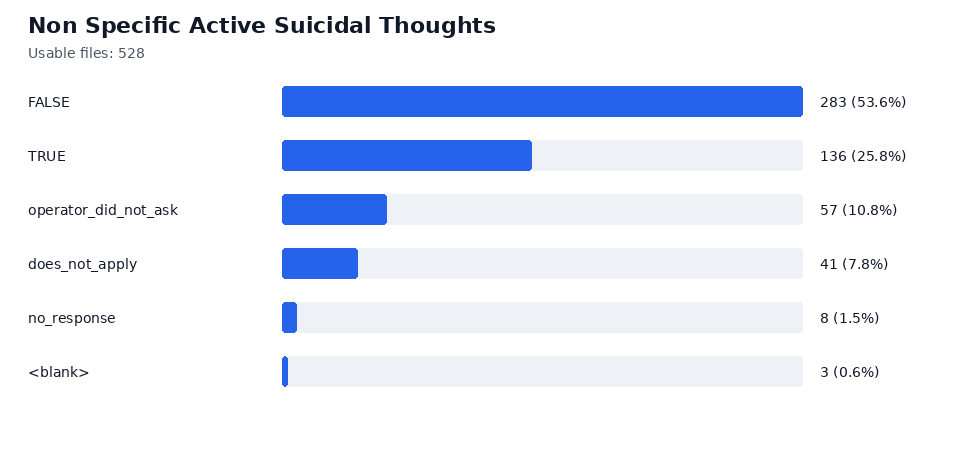
\includegraphics[width=0.95\linewidth]{usable_matches_distribution_plots/non_specific_active_suicidal_thoughts.png}
  \caption{Distribution of labels for \textit{Non Specific Active Suicidal Thoughts}.}
  \label{fig:non-specific-thoughts}
  \end{figure}

  \begin{figure}[htbp]
  \centering
  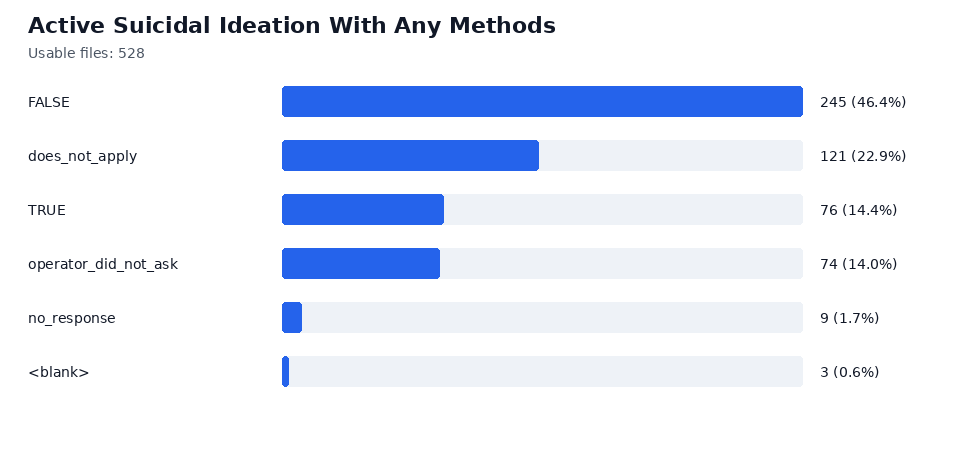
\includegraphics[width=0.95\linewidth]{usable_matches_distribution_plots/active_suicidal_ideation_with_any_methods.png}
  \caption{Distribution of labels for \textit{Active Suicidal Ideation With Any Methods}.}
  \label{fig:any-methods}
  \end{figure}

  \begin{figure}[htbp]
  \centering
  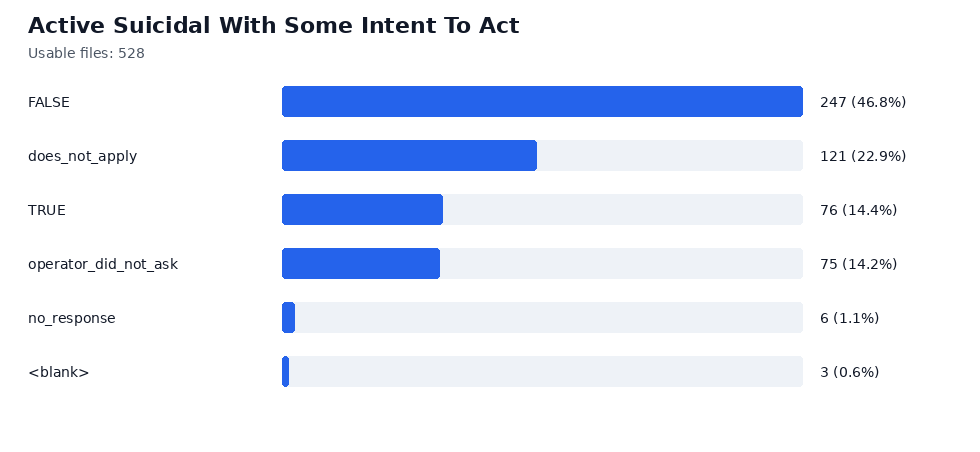
\includegraphics[width=0.95\linewidth]{usable_matches_distribution_plots/active_suicidal_with_some_intent_to_act.png}
  \caption{Distribution of labels for \textit{Active Suicidal With Some Intent To Act}.}
  \label{fig:some-intent}
  \end{figure}

  \begin{figure}[htbp]
  \centering
  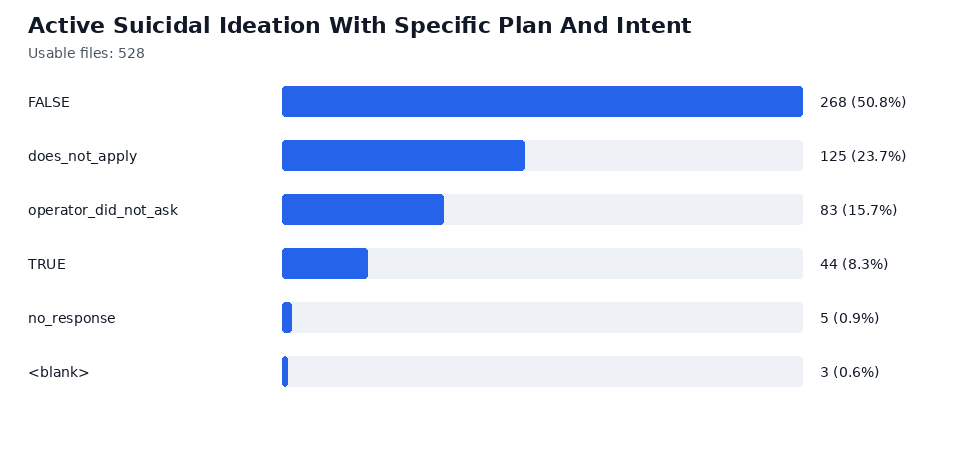
\includegraphics[width=0.95\linewidth]{usable_matches_distribution_plots/active_suicidal_ideation_with_specific_plan_and_intent.png}
  \caption{Distribution of labels for \textit{Active Suicidal Ideation With Specific Plan And Intent}.}
  \label{fig:specific-plan-intent}
  \end{figure}

  \begin{table}[htbp]
  \centering
  \small
  \begin{tabular}{llrr}
  \toprule
  \textbf{Prediction column} & \textbf{Most frequent label} & \textbf{Count} & \textbf{Percent} \\
  \midrule
  Wish To Be Dead & \texttt{false} & 212 & 40.15\% \\
  Non Specific Active Suicidal Thoughts & \texttt{false} & 283 & 53.60\% \\
  Active Suicidal Ideation With Any Methods & \texttt{false} & 245 & 46.40\% \\
  Active Suicidal With Some Intent To Act & \texttt{false} & 247 & 46.78\% \\
  Active Suicidal Ideation With Specific Plan And Intent & \texttt{false} & 268 & 50.76\% \\
  \bottomrule
  \end{tabular}
  \caption{Most frequent label for each AO--AS prediction target among the 528 usable text files.}
  \label{tab:label-distribution-summary}
  \end{table}

  For \textit{Wish To Be Dead}, the \texttt{true} (179, 33.90\%) and \texttt{false} (212, 40.15\%) cases are roughly balanced, with \texttt{false} being the most frequent
  label. For the other four prediction targets, the labels are imbalanced and the most frequent label is \texttt{false}. The most severe target,
  \textit{Active Suicidal Ideation With Specific Plan And Intent}, has only 44 \texttt{true} cases out of 528 usable examples.

  The labels also include non-binary response categories such as \texttt{operator\_did\_not\_ask}, \texttt{does\_not\_apply}, and \texttt{no\_response} (and a small
  number of blank cells). These categories should be clarified before model training, because they may need to be treated as separate classes, missing values, or mapped
  into binary labels. Among the 528 usable files, only 280 have all five labels expressed as pure \texttt{true}/\texttt{false} values.


\end{document}
